% vim: set tw=78 sts=2 sw=2 ts=8 aw et ai:

Having described our test environment, the current section will present the
results of our three scenarios illustrated above.

When testing locally using two loopback addresses our connection is ideal.
There is no intermediary networking equipment that can interfere with out
custom traffic. Our covert communication succeeds and we are able to send
commands successfully, while adhering to restrictions such as limited capacity
per packet and prohibition to run privileged commands.

\begin{figure}
  \centering
  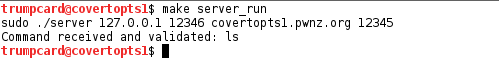
\includegraphics[width=0.5\textwidth]{img/server-run}
  \caption{Server Side Session}
  \label{fig:server-run}
\end{figure}

\begin{figure}
  \centering
  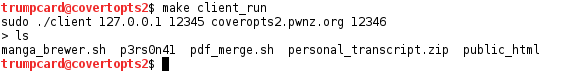
\includegraphics[width=0.5\textwidth]{img/client-run}
  \caption{Client Side Session}
  \label{fig:client-run}
\end{figure}

The second test we performed is whether a modern firewall equipment handles
our covert session differently. As can be seen from Figure
\ref{fig:server-run} and Figure \ref{fig:client-run}, Cisco ASA does not strip
or drop packets which use the TCP Alternate Checksum Data option. The
hostnames are conveniantly set to illustrate the two endpoints. It is worth
mentioning that we could not explore the full range of options such a
dedicated device offers, but we found no explicit feature that affects TCP
options directly.

Finally, we considered a real world test, between two public IPs. Despite our
previous tests were encouraging, we could not replicate the results in a real
world scenario. Since the intermediary devices are not under our control, we
cannot be certain that the root cause is explicit filtering of certain TCP
options or simply a default behaviour like the ones described in Subsection
\ref{sec:net-comm}. We cannot even determine the hardware platform of these
devices in order to speculate as to their prevalence on the Internet.

Overall, our solution has the capability to be deployed in real life, but its
effectiveness is highly dependent on the behavior of networking equipment
found between endpoints.
